% =====================================================================
% inspect-gate -- Journal of Intelligent Manufacturing (Springer) submission port.
%
% PROVENANCE: content ported byte-faithfully from ../paper.tex (source of
% truth; fixed and review-verified 2026-07-13). This is a PACKAGING port, not
% a rewrite: every content claim, number, and path is carried over unchanged.
% Structural changes only: Springer/JIM front matter (author-block placeholders,
% a 248-word abstract within JIM's live 150-250-word limit, 6 keywords within the
% live 4-6 requirement), a Springer "Declarations" section,
% and the removal of red \todo{} render blocks (see below).
%
% TEMPLATE STATUS: the official Springer Nature class (sn-jnl.cls) is NOT
% installed in this environment, and a single fetch attempt of
% https://static.springer.com/sn-article-template/sn-article-template.zip on
% 2026-07-13 returned a 404 HTML page (not a zip). This port therefore compiles
% in the standard "article" class, structured to Springer/JIM requirements.
% The sn-jnl drop-in is a MECHANICAL submission-day step:
%   \documentclass[sn-basic]{sn-jnl}  (or [pdflatex,sn-basic])
%   -> move title/author into \title{}\author{}\affil{} sn-jnl macros,
%   -> \keywords{...} instead of the \paragraph{Keywords} line below,
%   -> \bibliographystyle{sn-basic} (author-year, matching JIM's live house style)
%      instead of plainnat -- NOT the numbered variant (verified 2026-07-16 against
%      the live submission guidelines, which specify parenthetical author-year
%      in-text citation, e.g. "(Thompson, 1990)"),
%   -> declarations go under the sn-jnl "Declarations"/"\bmhead" convention.
% No content changes are needed for the drop-in; only these markup swaps.
%
% \todo RESOLUTION (submission port renders NO red TODO blocks): every red
% \todo{} from paper.tex has been converted to honest reviewer-facing prose in
% Limitations (Section~\ref{sec:limitations}); the underlying disclosures --
% which arms remain uncomputed -- are all preserved. The \todo macro below is
% neutralised (renders plain, no red) purely as a safety net.
% =====================================================================
\documentclass[11pt]{article}

\usepackage[utf8]{inputenc}
\usepackage[T1]{fontenc}
\usepackage[margin=1in]{geometry}
\usepackage{amsmath,amssymb}
\usepackage{graphicx}
\usepackage{booktabs}
\usepackage{array}
% JIM house style is author-year in parentheses, e.g. "(Thompson, 1990)" (live
% submission guidelines, link.springer.com/journal/10845/submission-guidelines,
% retrieved 2026-07-15); natbib's "round" option without "numbers" matches this.
\usepackage[round]{natbib}
\usepackage[hidelinks]{hyperref}
\usepackage{xcolor}
\usepackage{microtype}
\usepackage{placeins}
% Pack dedicated floats-only pages from the top instead of vertically
% centering/stretching them (kernel default \@fptop/\@fpsep/\@fpbot carry
% "plus Nfil" stretch designed for that centering; zeroing the stretch above
% and between floats removes dead white space on a page that is all floats).
\makeatletter
\setlength{\@fptop}{0pt}
\setlength{\@fpsep}{12pt plus 0fil}
\makeatother

% Neutralised in the submission port: all \todo disclosures were inlined into
% Limitations as prose. This definition is a safety net so a stray \todo, if
% any, renders as plain text rather than a red TODO block. Do NOT use it to add
% new gated content in this port.
\newcommand{\todo}[1]{#1}
% User-fill placeholder (author/declaration fields the submitter completes).
\newcommand{\userfill}[1]{\textit{[TODO-USER: #1]}}
\setlength{\parskip}{0.4em}

\title{A certified three-way triage gate for industrial visual inspection:
escaped-defect and false-reject guarantees on MVTec AD, VisA, and MPDD}

% --- Author block: Springer/JIM requires full names, affiliations, ORCID, and
% a corresponding author. Fill at submission; sn-jnl drop-in replaces these with
% \author[1]{...}\affil[1]{...}\email{...} macros. ---
\author{Zeyu Fu\thanks{\userfill{full author list, affiliations, ORCID iD(s),
and corresponding-author email/postal address.}}}
\date{\today}

\emergencystretch=3em
\begin{document}
\maketitle

\begin{abstract}
% Abstract word count: 248 (JIM live limit is 150-250 words; verified 2026-07-16,
% link.springer.com/journal/10845/submission-guidelines); claims mirror ../paper.tex verbatim.
% Descriptive nuances live in the body: PatchCore-on-VisA descriptive-only handling, Dinomaly
% published-figure gating, and the VisA 0.982->0.905 AUROC drop are all in Sec.~\ref{sec:repro}.
\noindent Anomaly detectors reach near-ceiling image-AUROC on MVTec AD, yet AUROC is not a
deployable decision: it names no operating threshold and bounds neither asymmetric-cost error ---
passing a defective part (an \emph{escaped defect}) or rejecting a good one (a \emph{false reject}).
We present \emph{inspect-gate}, a distribution-free triage layer sending each image to auto-pass,
auto-reject, or defer on any backbone's scores, with per-category certified escaped-defect
($P(\text{auto-pass}\mid\text{defective}) \le \alpha_{\text{miss}}$) and false-reject
($P(\text{auto-reject}\mid\text{good}) \le \alpha_{\text{fr}}$) rates. Both reduce exactly to
split-conformal calibration --- false-reject directly, escaped-defect through a score-negation
order-statistic identity --- adding no new estimator, inheriting finite-sample validity. A
category whose calibration pool is too small is \emph{refused} and reported
audited-not-certified, never rounded. Across two backbones and five
seeds, the machinery behaves as predicted, no kill-gate tripped. On MVTec AD,
escaped-defect certifies in all $15$ categories and false-reject in the four with enough
good-calibration data; a preregistered train-holdout remedy (PatchCore only) lifts false-reject to
$12$--$13$ of $15$, KS-failing categories audited-not-certified. On VisA both axes certify in all
$12$ categories, the validity audit passes non-vacuously in all
$120$ cells, and the deferral-skill audit becomes informative. A third benchmark, MPDD
(painted-metal parts), is the stingy extreme: its uniformly small good pools certify false-reject
in $0/6$ categories at the primary protocol (escaped-defect still $5/6$), and a flag-gated
train-holdout arm rescues $4/6$, with one KS-audited out, one below the calibration-pool
floor --- refusal tracking the data throughout ($0/6 \to 4/15 \to 12/12$). The confirmatory pooled-category
audit returns a constructive verdict on MVTec AD.
\end{abstract}

\paragraph{Keywords.} Industrial visual inspection \textperiodcentered{} Conformal prediction
\textperiodcentered{} Anomaly detection \textperiodcentered{} MVTec AD \textperiodcentered{} VisA
\textperiodcentered{} MPDD

\section{Introduction}
\label{sec:intro}

Automated visual inspection is one of the most mature industrial applications of computer vision,
and unsupervised anomaly detection (AD) on the MVTec AD benchmark~\citep{bergmann2019mvtec} is its
standard proving ground. Modern detectors --- memory-bank methods such as
PatchCore~\citep{roth2022patchcore} and reconstruction/transformer methods such as
Dinomaly~\citep{guo2025dinomaly} --- report image-level AUROC above $0.98$ and, for the newest
models, above $0.99$. On the usual reading the problem looks solved.

It is not solved as a decision. Image-AUROC is a threshold-free ranking summary: it says a
detector orders defective above good images well, but it names no operating point, and on a real
line an operating point is exactly what is needed. Worse, the two mistakes a threshold can make
are not symmetric. Passing a defective part (an \emph{escaped defect}) can ship a fault to a
customer; rejecting a good part (a \emph{false reject}) wastes yield and, at high rates, risks
eroding operator trust in the system. A useful inspection system must bound both, per
product category, with a guarantee that holds in finite samples rather than on average over an
idealized distribution.

We take the position that the deployable object is not a better detector but a certified
\emph{triage layer} on top of an existing one. Concretely, we route each image into three actions:
\emph{auto-pass} (confident-good, ship without review), \emph{auto-reject} (confident-defective,
scrap or rework without review), and \emph{defer} (send to a human). The value proposition is that
the two automated actions carry certificates: the auto-pass region is calibrated so that the
probability a truly defective image lands there is at most $\alpha_{\text{miss}}$, and the
auto-reject region so that the probability a truly good image lands there is at most
$\alpha_{\text{fr}}$; everything else defers. The human-review budget is then whatever the data
forces, and --- crucially --- it is visible: a category whose data cannot support the
requested guarantee defers more, rather than pretending to a certificate it cannot honor.
We evaluate the layer on three complementary benchmarks by design: MVTec AD, whose small
per-category good pools stress the refusal machinery; VisA, whose lower score ceilings and
larger good pools let both certificates bind everywhere and give the deferral-skill audit real
headroom; and MPDD (real painted-metal-parts fabrication), whose uniformly small good pools make
it the stingiest certifiability point --- false-reject certifiable in $0/6$ categories under the
primary protocol, the extreme that shows the gate refuses precisely when the data cannot pay for
a certificate.

This framing turns a benchmark score into an auditable decision and makes three contributions.

\begin{itemize}
  \item \textbf{A certified three-way triage system for inspection.} The contribution is not
        a new estimator --- both guarantees reduce exactly to split-conformal quantiles
        (Section~\ref{sec:gate}: false-reject directly, escaped-defect through a score-negation
        order-statistic identity) --- but the coupled system assembled from them: two
        simultaneously certified error axes (escaped-defect and false-reject), explicit
        per-category certifiability floors, first-class refusal, and the K1--K7 kill-gate battery,
        packaged as an auditable decision layer over any backbone's scores. To our knowledge no
        published method delivers this exact combination on MVTec AD or VisA; the binding K6
        pre-submission citation re-scan, executed 2026-07-13 (Section~\ref{sec:related}), returned a
        clear verdict --- no scoop. We foreground the ``no new math''
        property deliberately: it is what makes the guarantees finite-sample-exact and the tool a
        thin, testable wrapper rather than a heuristic.
  \item \textbf{Refusal as a first-class outcome, with teeth.} A per-category certifiability floor
        $\alpha_{\min}=1/(n_{\text{cal}}+1)$ makes ``we cannot certify this category at this rate''
        an explicit, reported state (audited-not-certified), never a silently loosened threshold.
        This is not cosmetic: on our own substrate (Table~\ref{tab:floors}), a non-refusing baseline
        that issues an auto-reject threshold and claims the requested false-reject rate
        $\alpha_{\text{fr}}=0.05$ in the $11$ categories the gate refuses would be asserting a
        guarantee the calibration pool cannot support --- the achievable floor there is
        $0.06$--$0.14$ (e.g.\ toothbrush $1/7=0.14$), $1.2\times$--$2.9\times$ looser than claimed --- so
        it silently over-promises where the gate refuses and defers. (On the escaped-defect axis the
        floor clears $\alpha_{\text{miss}}=0.10$ in all $15$ categories, so this failure mode does
        not arise there; a post-hoc binding demonstration (Section~\ref{sec:binding}) confirms this
        empirically --- in a range of (backbone, category) cells a non-refusing fixed-threshold
        baseline's \emph{realized} escaped-defect or false-reject rate exceeds the target while the
        certified gate holds within it on the same data.)
  \item \textbf{A practitioner-facing audit.} Beyond the certificate, we test whether
        field-standard threshold practice earns any deferral skill over honest random deferral
        (an excess-AURC audit), reporting a constructive or a debunking verdict symmetrically; the
        preregistered confirmatory pooled audit returns the constructive verdict --- practice earns
        real deferral skill in all five seeds (Section~\ref{sec:c2}).
\end{itemize}

Figure~\ref{fig:overview} summarizes the resulting pipeline, from a frozen backbone's per-image
score through the G1/G2 certificates and certifiability floor to the three-way auto-pass/defer/
auto-reject route.

\begin{figure}[htbp]
  \centering
  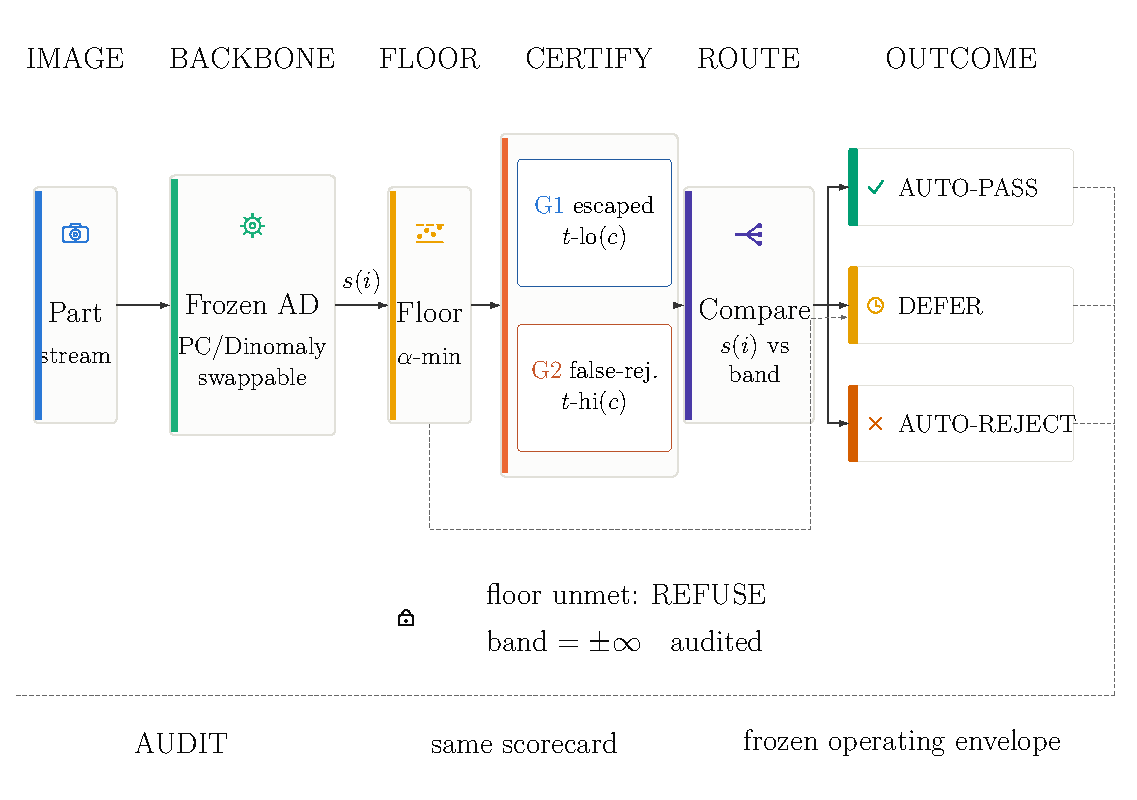
\includegraphics[width=0.8\linewidth]{../figures-src/fig-overview.pdf}
  \caption{Method overview. A frozen backbone (PatchCore or Dinomaly, interchangeable) scores each
  image; per-category calibration checks the certifiability floor
  $\alpha_{\min}=1/(n_{\text{cal}}+1)$ (Section~\ref{sec:floor}) and, when met, sets the G1
  escaped-defect threshold $t_{\text{lo}}(c)$ and the G2 false-reject threshold $t_{\text{hi}}(c)$
  (Section~\ref{sec:gate}). The three-way route then compares each score against
  $(t_{\text{lo}},t_{\text{hi}})$ to auto-pass, defer, or auto-reject, carrying the stated
  escaped-defect and false-reject guarantees; an unmet floor instead refuses the axis (band
  $=\pm\infty$), defers, and is reported audited-not-certified.}
  \label{fig:overview}
\end{figure}
\FloatBarrier

We are explicit about status. The preregistration was frozen on 2026-07-11 (sha256-pinned
sign-off; Section~\ref{sec:limitations}); this manuscript reports the primary-protocol axes on
all three benchmarks plus the frozen G2 train-holdout promotion arm and two \emph{post-freeze}
benchmarks (VisA and MPDD --- neither part of the frozen preregistration; both run under the
identical frozen protocol and code path, their audits reported as exploratory and never in the
confirmatory Holm family), and marks every remaining preregistered-but-uncomputed arm as an
explicit slot. No uncomputed result is presumed anywhere in the text.

\section{Related work}
\label{sec:related}

\paragraph{Distribution-free risk control.} The gate is an application of conformal
prediction~\citep{vovk2005algorithmic,lei2018distribution,angelopoulos2023gentle}: given an
exchangeable calibration set, an order statistic of the calibration scores yields a threshold with
a finite-sample coverage guarantee. The broader risk-controlling line ---
risk-controlling prediction sets~\citep{bates2021rcps} and Learn-then-Test~\citep{angelopoulos2021ltt}
--- generalizes this to bounding arbitrary monotone risks and to multiple-hypothesis calibration.
Our escaped-defect and false-reject bounds are the two one-sided special cases that split conformal
already delivers exactly (Section~\ref{sec:gate}); we deliberately use the simplest sufficient
construction rather than the more general RCPS/LTT machinery, and cite the latter as the family the
method belongs to.

\paragraph{Industrial anomaly detection.} MVTec AD~\citep{bergmann2019mvtec} defined the
per-category unsupervised setting we use. PatchCore~\citep{roth2022patchcore} (a coreset memory bank
over pretrained features) and Dinomaly~\citep{guo2025dinomaly} (a transformer reconstruction model)
are the two reproduced backbones here; EfficientAD~\citep{batzner2024efficientad} is a fast
alternative we discuss but do not certify (its only public implementations are community
reimplementations, so it cannot anchor a binding reproduction gate). Dinomaly descends from the
multi-class (one model, many categories) line initiated by UniAD~\citep{you2022unified} --- the
setting its published VisA figure reports and the one we use on VisA
(Section~\ref{sec:setup}). MPDD~\citep{jezek2021mpdd} adds a real painted-metal-parts fabrication
benchmark whose non-homogeneous backgrounds and small good pools make it a deliberately harsher
industrial-realism stress test than the two academic staples --- though, like them, still an
academic benchmark rather than production-line data (see Limitations, Section~\ref{sec:limitations}).
We use
anomalib~\citep{akcay2022anomalib} for the PatchCore implementation. Our contribution is orthogonal
to all of these: we consume their scores and add a decision layer, and we improve none of them.

\paragraph{Selective prediction and abstention.} The defer action is a selective-prediction
mechanism~\citep{geifman2017selective}, but applied at the decision layer with a two-sided,
per-category certificate rather than a single accuracy-coverage curve; the auto-reject certificate
(false-reject control) has no analogue in standard selective classification, which abstains only
around the positive decision.

\paragraph{Conformal anomaly detection and abstention.} Conformal methods have been applied to
anomaly detection before, but not to the certified inspection-triage decision we target. Early
work bounded false-alarm rates for sequential and trajectory
anomalies~\citep{laxhammar2011sequential,laxhammar2015inductive}; recent tooling controls the
false-discovery rate over flagged anomalies~\citep{hennhofer2026nonconform}; conformal risk
control~\citep{angelopoulos2022crc} and its graph instantiation
CRC-SGAD~\citep{bai2025crcsgad} bound a monotone risk (e.g.\ FNR/FPR) but emit a single flag, not
a three-way route; and dual-threshold conformal abstention for autonomous-system
perception~\citep{kumar2025beyond} adds a reject option on camera/LiDAR (and classification)
tasks, with no industrial-inspection estimand and no evaluation on MVTec AD. The closest
defect-detection application~\citep{shen2025conformal} bounds a single mean error rate for
surface-defect segmentation, again with no deferral option and not on MVTec AD. To our knowledge
no published method delivers a certified \emph{three-way} triage (auto-pass / auto-reject / defer)
on MVTec AD with \emph{coupled} escaped-defect and false-reject guarantees and explicit
per-category certifiability floors; the preregistered K6 scoop gate, run as a fresh pre-submission
re-scan on 2026-07-13, confirms this --- the closest published
systems~\citep{kumar2025beyond,bai2025crcsgad,shen2025conformal} each differ on a load-bearing axis
(substrate, estimand coupling, or the defer option), and two adjacent 2026 works (a selective-risk
certificate on generic vision, and a conformal cyber-physical-systems detector on sensor
time-series) target neither the image-inspection estimand nor the three-way route. That
is the seam this paper occupies. Section~\ref{sec:crcbaseline} instantiates the single-threshold
CRC construction~\citep{angelopoulos2022crc} as a quantitative baseline on our own canonical score
dumps under the identical protocol, isolating what the three-way route and its coupled
false-reject certificate add over the nearest single-flag alternative. More broadly, a recurring
reliability finding is that low
aggregate error coexists with brittle or miscalibrated decisions; our escaped-defect vs.\
false-reject framing is the industrial-inspection instance of that gap, and the excess-AURC audit
(Section~\ref{sec:audit}) tests whether standard thresholding beats chance at spending a deferral
budget.

\section{Methods}
\label{sec:methods}

\subsection{The three-way gate and its two certificates}
\label{sec:gate}

Each image $i$ in category $c$ has an anomaly score $s_i$ with the convention \emph{higher
$=$ more anomalous}. The gate is a pair of per-category thresholds $(t_{\text{lo}}(c),
t_{\text{hi}}(c))$ with $t_{\text{lo}} \le t_{\text{hi}}$: images with $s_i \le t_{\text{lo}}(c)$
auto-pass, images with $s_i \ge t_{\text{hi}}(c)$ auto-reject, and the rest defer. (If a refusal or
crossed thresholds leave the auto-reject band empty, the overlap simply defers, and both guarantees
still hold.)

\paragraph{G2 --- certified false-reject, directly.} $t_{\text{hi}}(c)$ is the split-conformal
upper quantile of the \emph{good} calibration scores at level $\alpha_{\text{fr}}$: with
$n_{\text{cal}}^{\text{good}}$ good calibration scores, it is the order statistic at rank
$\lceil (n+1)(1-\alpha_{\text{fr}}) \rceil$, guaranteeing $P(s \ge t_{\text{hi}} \mid \text{good})
\le \alpha_{\text{fr}}$ under exchangeability. This is exactly the split-conformal upper-quantile
construction applied to the good scores.
% implemented by the split-conformal routine relmetrics.conformal.SplitConformal

\paragraph{G1 --- certified escaped-defect, by negation.} Bounding
$P(s \le t_{\text{lo}} \mid \text{defective})$ is the mirror image: apply the same split-conformal
construction to the \emph{negated} defective calibration scores $Y=-X$ at level
$\alpha_{\text{miss}}$, then map the resulting upper quantile back through the negation. The gate
module proves this order-statistic identity, and it is checked against the design's
$\lfloor \alpha(n+1)\rfloor$ formula in the accompanying unit tests. No new
estimator is introduced; both certificates are the same conformal quantile.
% source: README.md "The gate: zero new math"; proof in inspect_gate/gate.py module docstring; checked in tests/test_gate.py

\paragraph{Mondrian per-category stratification.} Calibration is stratified by category (a Mondrian
conformal construction): each category gets its own $(t_{\text{lo}}, t_{\text{hi}})$, so the
guarantee is conditional on category, not marginal. An optional finer per-defect-type
stratification is exploratory only (Section~\ref{sec:limitations}).

\subsection{Certifiability floors and refusal}
\label{sec:floor}

Split conformal cannot certify an arbitrarily small rate from a finite calibration pool: the
smallest achievable level is $\alpha_{\min} = 1/(n_{\text{cal}}+1)$. A category is certifiable for a
guarantee iff $\alpha_{\min} \le \alpha$; otherwise the gate \emph{refuses}, setting the
corresponding threshold to $\pm\infty$ (the band is empty, all such images defer) and marking the
category audited-not-certified for that axis. Refusal is emitted, never rounded away
% source: PREREG-DRAFT-2026-07-10.md §2--§3 (alpha_min = 1/(n_cal+1)); README.md "Honest-uncertainty rules"
--- this is the honesty rule that makes the floor table (Section~\ref{sec:floors}) a result rather
than a limitation.

\subsection{Validity audit (V1) and kill-gates (K1--K7)}
\label{sec:v1}

We fix $\alpha_{\text{miss}}=0.10$ and $\alpha_{\text{fr}}=0.05$ throughout, with a $+3$pp
estimator tolerance (thresholds $0.13$ / $0.08$) and $95\%$ one-sided Clopper--Pearson
intervals~\citep{clopper1934use}.
% source: PREREG-DRAFT-2026-07-10.md §2 (frozen targets table)
The \emph{validity audit} V1 has two tiers. Tier-1 checks that the realized mean escaped-defect and
false-reject rates lie within target$+3$pp over repeated calibration/evaluation splits; this is the
certificate-validity statistic. Tier-2 forms a Clopper--Pearson upper bound and is graded, per the
frozen amendments, as a stringent estimator-variance readout (Section~\ref{sec:tier2verdict}),
because on MVTec AD its power floor is not met per repeat and its tolerance is near-unpassable by
construction for a correctly-calibrated gate.

A battery of preregistered kill-gates guards the construction: K1 (coverage sanity --- halt if
tier-1 fails in $\ge 5$ of the $15\!\times\!B$ cells), K2 (vacuity --- kill if median deferral
$>0.80$ in $\ge 8/15$ categories on all backbones), K3 (backbone floor --- mean image-AUROC
$\ge 0.90$), K4 (audit headroom), K5 (calibration floor --- fires only if $\alpha_{\min}>0.10$ in
$\ge 3$ categories), K6 (a citation re-scan for a prior certified triage), and K7 (a compute guard).
% source: PREREG-DRAFT-2026-07-10.md §5, §7.1 (falsification conditions)

\subsection{Excess-AURC audit}
\label{sec:audit}

Beyond validity, we ask whether standard thresholding practice earns deferral skill at all.
For each practice --- B1 (global fixed threshold), B2 (per-category tuned), B3 (train-good quantile)
--- we compare its area-under-the-risk-coverage-curve against the closed-form random-deferral null
(evaluated in closed form, never Monte-Carlo'd), using a matched-abstention,
% closed-form random-deferral AURC null: relmetrics.aurc.random_aurc
category-stratified permutation $p$-value ($2000$ permutations), a category-blocked bootstrap CI,
and a roster-derived Holm~\citep{holm1979simple} correction. The verdict is symmetric: if no
practice beats random the paper reports a debunking finding; if all do it reports a constructive one.
% source: PREREG-DRAFT-2026-07-10.md §7 step 7; README.md audit.py

\section{Experimental setup}
\label{sec:setup}

\paragraph{Data.} Three public benchmarks. MVTec AD~\citep{bergmann2019mvtec}, staged from a fixed
tarball (\texttt{sha256\,=\,cf4313b1\allowbreak\ldots98cd3d}): $15$ object/texture categories, $3{,}629$
train-good images, and a test set of $467$ good $+$ $1{,}258$ defective $=$ $1{,}725$ images
across $73$ defect types. VisA~\citep{zou2022spot}, staged from the official
\texttt{VisA\_\allowbreak 20220922} archive under the official \texttt{spot-diff} $1$-class split:
$12$ categories, $8{,}659$ train-good images, and a test set of $962$ good
$+$ $1{,}200$ anomalous $=$ $2{,}162$ images (VisA's public ground truth carries a single
``bad'' stratum per category, so the defect-type Mondrian axis is unavailable there). MPDD~\citep{jezek2021mpdd}
(post-freeze exploratory; see below), $6$ real painted-metal-part categories in native MVTec-AD
directory layout, staged from the credential-free public HuggingFace mirror \texttt{meksamiao/mpdd}
(\texttt{archive\ sha256\,=\,69f8da73\allowbreak\ldots ddd6}, recorded in the frozen split manifest):
$888$ train-good images and a test set of $176$ good $+$ $282$ defective $=$ $458$ images. Both box
layouts (MVTec AD, VisA) were built by symlinking the official split file,
refusing on any count mismatch; for MPDD, which ships without an external split file, the ground-truth
test split is a frozen per-category manifest generated from the verified staged tree (the role
the official one-class split file plays for VisA). The score dumps were adapted to the canonical schema with a
per-image join against that split that refuses on any missing or extra image.
% official 1-class split file: 1cls.csv; box builder: orchestration/visa_prep.py;
% score-dump adapter: visa_results_2026-07-12/scripts/visa_adapter.py
% MPDD source + sha256: DATA_MANIFEST.md (meksamiao/mpdd, archive_sha256 in mpdd_split_manifest.json);
% MPDD adapter: mpdd_results_2026-07-13/scripts/mpdd_adapter.py -> ADAPTER-REPORT.json
% source: PREREG-DRAFT-2026-07-10.md §2 (data provenance); §7 step 1;
% visa_results_2026-07-12/ADAPTER-REPORT.json (official_test_counts)
\paragraph{Backbones (Branch A, $B=2$).} PatchCore~\citep{roth2022patchcore} via
anomalib~\citep{akcay2022anomalib} (a Wide ResNet-50-2 backbone, features from the second and
third stages, coreset ratio $0.10$)\footnote{The reproduction target $0.991$ is PatchCore's published
\emph{25\%-coreset} mean image-AUROC (the paper's own headline is ``up to $99.6\%$''); our
scoring uses the $10\%$-coreset configuration (PREREG D3), a different published operating point
in the same paper. The frozen $\pm 0.02$ tolerance spans the gap and the gate passes with margin
either way (Table~\ref{tab:repro}).} and Dinomaly~\citep{guo2025dinomaly} (canonical score dump,
its own eval script; on VisA, the reference repo's multi-class setting --- one model per seed for
all $12$ categories --- which is the setting its published VisA figure reports). Both were
confirmed present and reproduction-passing before any calibration, so the preregistered
two-backbone branch (Branch A) is active; the same two backbones and configurations are used
unchanged on VisA.
% source: PREREG-DRAFT-2026-07-10.md §1--§2; ANALYSIS-MEMO.md §1
\paragraph{Protocol.} Primary protocol: test-side good calibration, no
train-holdout. For each (backbone, category, seed) we draw $R=20$ stratified $50/50$
% primary-protocol CLI flag: --good-cal test
calibration/evaluation splits (split-seed $=$ repeat index), with $5$ backbone seeds ($0$--$4$).
% source: PREREG-DRAFT-2026-07-10.md §2 (split protocol)

\section{Results}
\label{sec:results}

All numbers in this section are recomputed from the frozen local score dumps by the archived
analysis pipeline --- a MVTec AD analysis stage, a stage-identical VisA analysis stage, a
stage-identical MPDD analysis stage (with its own train-holdout rescue stage), and the
G2-promotion stage, each emitting a frozen result summary; none is trusted from a training log or
the literature.
% MVTec: analysis_2026-07-10/scripts/run_analysis.py -> analysis_2026-07-10/SUMMARY.json;
% VisA: visa_results_2026-07-12/scripts/run_visa_analysis.py -> visa_results_2026-07-12/SUMMARY.json;
% MPDD: mpdd_results_2026-07-13/scripts/run_mpdd_analysis.py -> SUMMARY.json;
%       mpdd_results_2026-07-13/scripts/run_mpdd_holdout_analysis.py -> HOLDOUT-RESULTS.json;
% G2 promotion: g2_promotion_2026-07-12/run_g2_promotion.py

\subsection{Reproduction gate}
\label{sec:repro}

On all three benchmarks the gate recomputes image-AUROC (Mann--Whitney rank-sum identity) directly
from the local scores and compares it against a named published target (Table~\ref{tab:repro}).
On MVTec AD both backbones pass in all $5$ seeds, and K3 (mean AUROC $\ge 0.90$) holds with wide
margin. On VisA, Dinomaly passes in all $5$ seeds against its own published VisA figure
($0.987$, multi-class setting), and our recomputation again reproduces its reported per-seed
mean image-AUROC seed for seed (max per-category deviation $3.3\times 10^{-5}$ over
% reproduced value: the training-log "Mean: I-Auroc" line
all $60$ seed$\times$category cells). PatchCore has no repo-confirmed published VisA figure, so
per the tool's no-guessed-target rule its VisA row is \emph{descriptive} (no pass/fail is
graded); its recomputed mean of $0.903$--$0.908$ still clears the K3 floor, though with thin
margin (seed $3$: $0.9033$, i.e.\ $0.33$pp above the $0.90$ floor), and the drop from $0.982$
(MVTec) is exactly the lower-ceiling substrate the audit needs (Section~\ref{sec:auditres}). On
MPDD, Dinomaly passes in all $5$ seeds against its published MPDD multi-class figure ($0.972$;
recomputed mean $0.9712$--$0.9738$, grand mean $0.9722 \pm 0.0010$), our recomputation matching
the box's per-category training-log AUROC to $\le 4.9\times10^{-5}$; PatchCore-on-MPDD has no
repo-confirmed published figure, so per the same no-guessed-target rule its row is
descriptive (recomputed mean $0.948$--$0.957$).
% source: analysis_2026-07-10/SUMMARY.json["reproduction"]; ANALYSIS-MEMO.md §1;
% visa_results_2026-07-12/SUMMARY.json["reproduction"]; ADAPTER-REPORT.json (xcheck)
% MPDD: mpdd_results_2026-07-13/SUMMARY.json["reproduction"] (+seed_stability_summary);
%   ADAPTER-REPORT.json (auroc_xcheck max_abs_diff 4.9e-5; per-seed maxima 4.3/4.4/3.2/4.9/4.9e-5)

\begin{table}[t]
  \centering
  \caption{Reproduction gate, $5$ seeds per backbone per benchmark. Mean image-AUROC range is
  over seeds; the weakest category is named. ``n/a'': no repo-confirmed published
  PatchCore-on-VisA/MPDD figure exists, so that row is descriptive by design (no pass/fail graded).
  Recomputed from the frozen MVTec AD, VisA, and MPDD analysis summaries.}
  % source: analysis_2026-07-10, visa_results_2026-07-12, mpdd_results_2026-07-13 SUMMARY.json["reproduction"]
  \label{tab:repro}
  \small
  \begin{tabular}{l l c >{\raggedright\arraybackslash}p{0.15\textwidth} >{\raggedright\arraybackslash}p{0.18\textwidth} c}
    \toprule
    Benchmark & Backbone & Target ($\pm 0.02$) & Mean I-AUROC (seed range) & Weakest category & Gate \\
    \midrule
    MVTec AD & PatchCore & 0.991 & 0.9817--0.9826 & toothbrush 0.911--0.917 & PASS 5/5 \\
    MVTec AD & Dinomaly  & 0.996 & 0.9957--0.9965 & capsule 0.976--0.982    & PASS 5/5 \\
    VisA     & PatchCore & n/a   & 0.9033--0.9083 & macaroni2 0.656--0.665  & descriptive \\
    VisA     & Dinomaly  & 0.987 & 0.9866--0.9876 & macaroni2 0.956--0.966  & PASS 5/5 \\
    MPDD     & PatchCore & n/a   & 0.9481--0.9568 & bracket black 0.872--0.888 & descriptive \\
    MPDD     & Dinomaly  & 0.972 & 0.9712--0.9738 & bracket black 0.929--0.940 & PASS 5/5 \\
    \bottomrule
  \end{tabular}
\end{table}
\FloatBarrier

\subsection{Cross-seed stability}
\label{sec:seed}

PatchCore's five seeds are genuinely distinct: all $60$ seed-0-vs-seed-$N$ score-table comparisons
($15$ categories $\times$ $4$ seeds) are $0/60$ bit-identical, with $\max|\Delta\text{score}|$
ranging $0.026$--$0.153$ (mean $0.074$) --- a real but modest variance source, so PatchCore is
reported as a $5$-effective-seed backbone, not collapsed to one. Dinomaly is low-variance: mean
image-AUROC across seeds $0.9960 \pm 0.00029$, with the widest per-category spread only $0.0060$
(capsule). The same picture holds on VisA: PatchCore is $0/48$ bit-identical
($\max|\Delta\text{score}|$ $0.044$--$0.256$), and Dinomaly's mean image-AUROC across seeds is
$0.9870 \pm 0.0004$ with the widest per-category spread $0.0104$ (macaroni2). On MPDD the pattern
repeats once more: PatchCore is $0/24$ bit-identical across the seed-0-vs-seed-$N$ comparisons,
and Dinomaly's mean image-AUROC across seeds is $0.9722 \pm 0.0010$.
% source: analysis_2026-07-10/SUMMARY.json["seed_stability_summary"]; ANALYSIS-MEMO.md §2;
% visa_results_2026-07-12/seed_stability/seed_stability.json;
% mpdd_results_2026-07-13/SUMMARY.json["seed_stability_summary"]

\subsection{Certifiability floors and the G1/G2 split}
\label{sec:floors}

Table~\ref{tab:floors} is the paper's honesty figure. The per-category calibration counts computed
from the full local test arrays match the preregistered arithmetic-only floor table exactly
($0/15$ mismatches for both backbones, identical across all $5$ seeds). At the frozen rates,
escaped-defect (G1) is certifiable in all $15$ categories; false-reject (G2) is certifiable
in exactly $4$ --- cable, hazelnut, screw, transistor --- the categories with
$n_{\text{cal}}^{\text{good}} \ge 19$. The other $11$ categories are refused for G2 and reported
audited-not-certified. We are careful about what this exact match does and does not show: the
per-category counts are a \emph{deterministic} function of the fixed MVTec test split
(round-half-to-even of $n/2$), so the $0/15$ agreement with the preregistered table is a
pipeline-correctness check --- it confirms the data staging re-derives the frozen counts with no
off-by-one or CSV-read error --- not an empirical result about the gate. The genuinely empirical
result is the V1 tier-1 validity audit below (Section~\ref{sec:v1res}), measured from real
calibrate/route/evaluate runs, which could have failed had the calibration or routing pipeline been
broken.
% source: PREREG-DRAFT-2026-07-10.md §3 (floor table); SUMMARY.json["n_cal_count_mismatches_across_seeds"]=0; ANALYSIS-MEMO.md §3

\begin{table}[t]
  \centering
  \small
  \caption{Per-category certifiability at $\alpha_{\text{miss}}=0.10$, $\alpha_{\text{fr}}=0.05$
  (backbone-invariant; pure functions of the shared MVTec test split). G1 certifies in $15/15$,
  G2 in $4/15$. Source: the frozen preregistration (\S3), reproduced with $0/15$ mismatch by the
  analysis pipeline.}
  % source: PREREG-DRAFT-2026-07-10.md §3; recomputed by run_analysis.py
  \label{tab:floors}
  \begin{tabular}{lccccc}
    \toprule
    Category & $n_{\text{cal}}^{\text{def}}$ & $\alpha_{\min}$(G1) & G1@0.10 & $n_{\text{cal}}^{\text{good}}$ & G2@0.05 \\
    \midrule
    bottle     & 32 & 0.0303 & OK & 10 & REFUSE \\
    cable      & 46 & 0.0213 & OK & 29 & OK \\
    capsule    & 54 & 0.0182 & OK & 12 & REFUSE \\
    carpet     & 44 & 0.0222 & OK & 14 & REFUSE \\
    grid       & 28 & 0.0345 & OK & 10 & REFUSE \\
    hazelnut   & 35 & 0.0278 & OK & 20 & OK \\
    leather    & 46 & 0.0213 & OK & 16 & REFUSE \\
    metal\_nut & 46 & 0.0213 & OK & 11 & REFUSE \\
    pill       & 70 & 0.0141 & OK & 13 & REFUSE \\
    screw      & 60 & 0.0164 & OK & 20 & OK \\
    tile       & 42 & 0.0233 & OK & 16 & REFUSE \\
    toothbrush & 15 & 0.0625 & OK & 6  & REFUSE \\
    transistor & 20 & 0.0476 & OK & 30 & OK \\
    wood       & 30 & 0.0323 & OK & 10 & REFUSE \\
    zipper     & 60 & 0.0164 & OK & 16 & REFUSE \\
    \midrule
    \multicolumn{3}{l}{\textbf{Certifiable}} & 15/15 & & 4/15 \\
    \bottomrule
  \end{tabular}
\end{table}
\FloatBarrier

\paragraph{VisA: the same arithmetic, a friendlier split.} On VisA the identical floor
computation lands on the opposite side of the ledger: every category's test split carries
$100$ anomalous and $50$--$101$ good images, so after the $50/50$ calibration split
$n_{\text{cal}}^{\text{def}} = 50$ everywhere ($\alpha_{\min}^{\text{G1}} = 0.0196$) and
$n_{\text{cal}}^{\text{good}} \in \{25, 30, 50\}$ ($\alpha_{\min}^{\text{G2}} =
0.0196$--$0.0385$), all below $\alpha_{\text{fr}} = 0.05$. G1 and G2 both certify in
$12/12$ categories under the primary protocol alone --- no train-holdout remedy is needed on
VisA --- and the floors are again identical across both backbones and all five seeds ($0$
mismatches). This is the refusal mechanism working in both directions: it refuses $11/15$
categories on MVTec AD because the data cannot support the rate, and certifies $12/12$ on VisA
because it can.
% source: visa_results_2026-07-12/gate_calibration/v1_*_seed*.json ("certifiability_floors");
% SUMMARY.json["n_cal_count_mismatches_across_seeds"]=0

\paragraph{MPDD: the stingy extreme of pool-size-driven refusal.} MPDD's per-category
test-good pools are uniformly small ($26$--$32$ images $\to n_{\text{cal}}^{\text{good}}$
$13$--$16$, every one below the $19$ the false-reject floor needs at $\alpha_{\text{fr}}=0.05$),
so G2 is certifiable in $0/6$ categories under the primary protocol, on both backbones,
identical across all five seeds ($0$ mismatches). G1 (escaped-defect) stays healthy at $5/6$ ---
only connector fails, its $14$ test-defective yielding $n_{\text{cal}}^{\text{def}}=7<9$.
This places MPDD at the stingy end of three points consistent with pool-size-driven refusal, ordered by good-pool size:
MPDD $0/6 \to$ MVTec AD $4/15 \to$ VisA $12/12$ (all three computed apples-to-apples by
the identical floor code path). MPDD is thus not an intermediate point but the cleanest
demonstration of the paper's thesis --- the certifiable count is a property of how much
exchangeable good data the protocol can spend, and the gate refuses precisely when the data
cannot pay for a $5\%$-false-reject certificate.
% source: mpdd_results_2026-07-13/SUMMARY.json["g2_certifiable_count"]={patchcore:0,dinomaly:0},
%   ["n_cal_count_mismatches_across_seeds"]=0; gate_calibration/v1_*_seed0.json (G1 5/6, connector);
%   FLOOR-PREDICTION.md (trend MPDD 0/6 -> MVTec 4/15 -> VisA 12/12)
Figure~\ref{fig:categorymap} makes this certify-or-refuse pattern visible at the category level
across all three benchmarks: VisA certifies both axes in every category, MVTec AD's false-reject
row is hatched (refused) everywhere except the four categories in Table~\ref{tab:floors}, and
MPDD's false-reject row is hatched throughout --- the visual complement of the same table.

\begin{figure}[htbp]
  \centering
  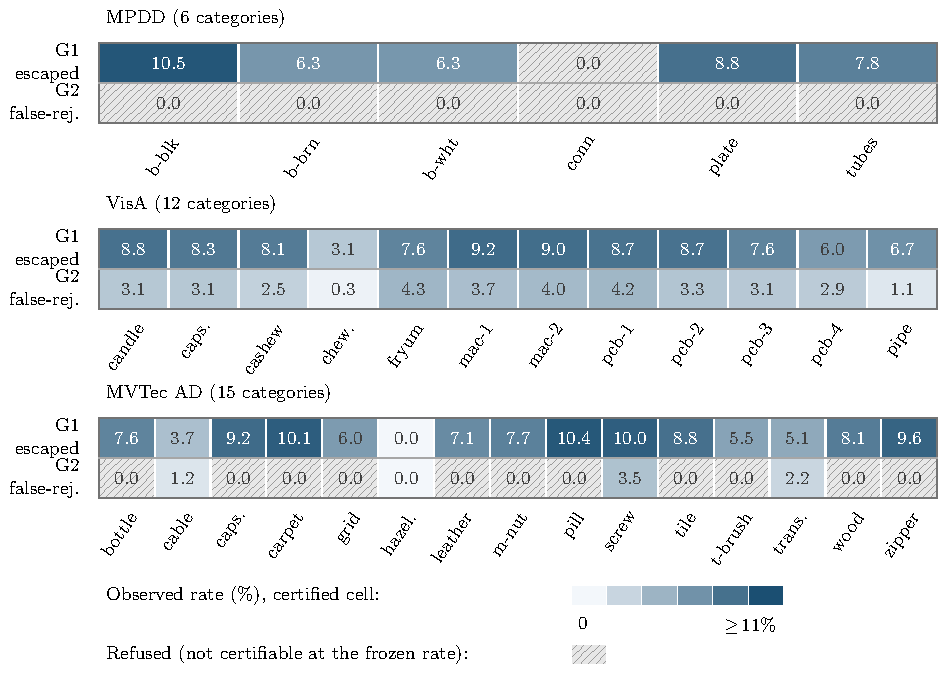
\includegraphics[width=\linewidth]{../figures-src/fig-categorymap.pdf}
  \caption{Per-category certification map for escaped-defect (G1) and false-reject (G2) at the
  frozen rates ($\alpha_{\text{miss}}=0.10$, $\alpha_{\text{fr}}=0.05$), pooled over both backbones
  and five seeds, for MPDD, VisA, and MVTec AD. Colored cells are certified, shaded by the observed
  rate; hatched gray cells are refused as not certifiable at the frozen rate under the primary
  protocol (all of MPDD's G2 column, MPDD's connector on G1, and the $11/15$ MVTec AD categories
  below the false-reject floor in Table~\ref{tab:floors}).}
  \label{fig:categorymap}
\end{figure}
\FloatBarrier

\subsection{G2 train-holdout promotion on MVTec AD (frozen remedy arm)}
\label{sec:g2promo}

The preregistered calibration-efficiency remedy --- recalibrating G2 on held-out
\emph{train}-good scores, gated behind a per-category KS exchangeability test with a mandatory
audited-not-certified fallback --- was computed on 2026-07-12 under the 2026-07-11 freeze,
for PatchCore only: Dinomaly has no train-side score dump (its reference eval scores
test images only), so the promotion arm is single-backbone by construction, disclosed here
rather than implied otherwise. It behaves as preregistered: G2-certifiable categories rise from
$4/15$ to $13/15$ in seeds $0$--$3$ and $12/15$ in seed $4$. The KS gate does real work rather than rubber-stamping:
leather fails it in all five seeds (its train-good and test-good score distributions are not
exchangeable) and screw additionally fails in seed $4$ --- each is reported
audited-not-certified, never silently promoted, and the seed-$4$ screw case shows a category
certified under the primary protocol can still be \emph{refused} under the holdout arm when
exchangeability breaks. Toothbrush remains uncertifiable at $\alpha_{\text{fr}}=0.05$ under both
arms, exactly as preregistered ($n^{\text{good}}$ too small in either pool). K1 is not tripped
in any promoted seed aggregate.
% source: g2_promotion_2026-07-12/G2-PROMOTION-RESULT.json (summary + compare);
% SIGN-OFF-RECORD-2026-07-11.md (freeze); PREREG-DRAFT-2026-07-10.md §3.1/§8

\subsection{MPDD train-holdout rescue (post-freeze exploratory)}
\label{sec:mpddholdout}

We report the primary-protocol $0/6$ of the preceding section as MPDD's thesis-confirming
headline; the train-holdout arm below is a clearly secondary, post-freeze, PatchCore-only result.
The train-holdout calibration-efficiency lever the frozen MVTec remedy exercises
(Section~\ref{sec:g2promo}) turns MPDD's $0/6$ primary refusal into a $4/6$ rescue, a vivid
single-benchmark illustration of the same lever. MPDD's train-good pools are large ($54$--$289$ per category) where its
test-good pools are tiny, so recalibrating G2 on a $20\%$ held-out train-good pool (the flag-gated
train-holdout calibration mode, $20\%$ holdout fraction; PatchCore only, as on
MVTec --- Dinomaly dumps no train-side scores, so the arm is single-backbone by construction)
clears the false-reject floor for the $5/6$ categories whose holdout pool reaches $n\ge 19$. The
same per-category KS exchangeability gate then adjudicates each promotion, and it does decisive
work: G2-certifiable rises from $0/6$ to $4/6$, identical in all five seeds. Two
categories are honestly held back --- metal plate, whose holdout pool ($11$) is still
below the floor, and tubes, which fails the KS gate (BH-adjusted $p\approx
1.2\times10^{-5}$; its train-good and test-good score distributions are demonstrably
non-exchangeable) and is reported audited-not-certified rather than promoted. The remaining four
(bracket black, bracket brown, bracket white, connector)
promote cleanly (KS $p_{\text{BH}}\ge 0.44$ every seed). Connector is the one category
G1 refuses under the primary protocol ($n_{\text{cal}}^{\text{def}}=7<9$ defective) yet
the arm G2-certifies (holdout-good $26\ge 19$): the two certificates gate on independent sample
axes --- defect count for escaped-defect, good count for false-reject --- so this is coherent, not
contradictory. Its $100\%$ deferral (the highest of any category, since G1 refusal leaves the
auto-reject band empty) nonetheless makes that G2 certificate operationally hollow in practice.
So the count-only floor of $5/6$ is
audited down to a genuinely certified $4/6$ --- the KS guardrail keeping the rescue honest, exactly
the exchangeability risk MPDD's non-homogeneous backgrounds were expected to pose. As a sanity
check (no gate), the holdout arm's $80\%$-memory-bank test scores rank-correlate with the primary
$100\%$-bank scores at Spearman $\rho\ge 0.918$ across all $6\times5$ category-seed cells (max
$|\Delta\text{image-AUROC}|=0.040$), confirming the same model was scored. This arm is post-freeze
exploratory and flag-gated prereg-neutral (it re-freezes nothing and is never in the confirmatory
Holm family); the $0/6 \to 4/6$ contrast on the same benchmark and the same scores is a vivid
single-benchmark demonstration of the calibration-efficiency lever. The larger, \emph{confirmatory}
instance of the same lever is the frozen MVTec train-holdout remedy (Section~\ref{sec:g2promo}),
which lifts G2 from $4/15$ to $12$--$13/15$ across seeds ($13$ in seeds $0$--$3$, $12$ in seed~$4$).
The primary-protocol $0/6$ stays the honest headline for this industrial benchmark: on real metal
parts the gate certifies nothing at the $5\%$ false-reject budget because the data cannot pay for
it --- exactly what a refusal-first design should do.
% source: mpdd_results_2026-07-13/HOLDOUT-RESULTS.json (summary: g2_certified_by_seed=4 all seeds,
%   floor-only prediction 5/6, tubes KS p_bh 1.2e-5, metal_plate n=11<19, min Spearman 0.9186,
%   max|auroc_delta| 0.0399); run_mpdd_holdout_analysis.py

\subsection{Validity audit V1 (tier-1) and the kill-gates}
\label{sec:v1res}

Per frozen amendment A3, tier-1 is reported \emph{per axis}, with the false-reject axis
evaluated only over G2-certified cells: wherever G2 is refused the auto-reject region is empty
and the measured false-reject rate is identically $0$ --- a pass without evidence that A3
excludes from every count. On the escaped-defect axis, tier-1 passes in all $150$
MVTec cells ($2$ backbones $\times 5$ seeds $\times 15$ categories), all $120$
VisA cells ($2 \times 5 \times 12$), and all $60$ MPDD cells ($2 \times 5 \times 6$),
every rate within target$+3$pp. On the false-reject
axis, MVTec has $40$ evaluable cells ($4$ G2-certified categories $\times 2 \times 5$) and
passes $40/40$, with the other $110$ cells reported G2-REFUSED and excluded; on VisA
every category is G2-certified, so all $120/120$ cells are evaluable and pass
non-vacuously; on MPDD every category is G2-refused under the primary protocol, so all $60$
false-reject cells are G2-REFUSED and excluded (the mirror image of VisA, and the primary-protocol
counterpart to the train-holdout rescue of Section~\ref{sec:mpddholdout}). Tier-1 is a necessary-not-sufficient pipeline check --- a conservative gate
realizes rates well below target, so passing validates the calibrate/route/evaluate machinery
rather than demonstrating sharpness. Consequently K1 is not tripped (the A3 exclusion
cannot change K1's count: excluded cells cannot fail) ($0$ violations in every
(backbone, seed) aggregate, against the $5$-cell MVTec/VisA kill threshold and, on MPDD, against
a proportionally-scaled $2$-cell threshold\footnote{At $n_{\text{cat}}=6$ the design's absolute
kill thresholds (max $5$ violations, min $8$ categories) are vacuously un-trippable, so on MPDD
they are scaled to the design's proportions --- $5/15\to\lceil 6/3\rceil=2$ for K1 and
$8/15\to\lceil 6\cdot 8/15\rceil=4$ for K2 --- with the raw counts recorded so any threshold is
re-derivable. The no-trip verdict is invariant to the rounding rule: any reasonable rounding of
the proportional thresholds gives the same outcome ($0$ violations and $\le 2$ vacuous categories
clear even the tightest rounding). These diagnostic kill-gates are never part of the confirmatory family.}) and K2 is
not tripped (on MVTec/VisA at most $1$ vacuous category --- VisA/PatchCore/seed~$2$ --- against the
$8$-category/$0.80$-deferral threshold; on MPDD at most $2$ vacuous categories per aggregate
against the scaled $4$-category threshold), in all $30$ aggregates across the three
benchmarks (Table~\ref{tab:v1}). Median per-category deferral at seed $0$ on MVTec AD is
$70.0\%$ for PatchCore (mean $55.1\%$; max pill $78.0\%$, min transistor $2.0\%$) and $69.5\%$
for Dinomaly (mean $54.2\%$; max capsule $77.3\%$, min screw $3.1\%$) --- elevated because G2 refusal
empties the auto-reject band in $11/15$ categories, but far from the vacuity threshold. On VisA,
where G2 certifies everywhere and the auto-reject band is live in every category, seed-$0$
median deferral drops to $18.7\%$ for PatchCore (max macaroni2 $72.5\%$, min chewinggum
$2.0\%$) and $4.2\%$ for Dinomaly (max capsules $21.9\%$, min candle $2.5\%$) --- direct
operational evidence that the elevated MVTec deferral was the price of honest G2 refusal, not a
property of the gate. MPDD sits at the far end again: with G2 refused in all $6$ categories under
the primary protocol, seed-$0$ median deferral is $74.1\%$ for PatchCore (max connector $100\%$,
min bracket brown $61.8\%$) and $70.9\%$ for Dinomaly (max connector $100\%$, min bracket white
$53.3\%$), the highest of the three benchmarks and exactly what $0/6$ certification predicts.
These are three honest operating points, not a defect and a fix: MPDD's $\sim 72\%$ and the
$55$--$70\%$ MVTec deferral are the cost of refusing to certify small good-calibration pools,
and VisA's $4$--$19\%$ is what the same gate, same code path, spends when the good pools are large
enough to certify every category.
% source: analysis_2026-07-10/SUMMARY.json["gate_calibration_k1_k2"]; ANALYSIS-MEMO.md §3;
% visa_results_2026-07-12/SUMMARY.json["gate_calibration_k1_k2"] + gate_calibration/v1_*_seed0.json
% MPDD deferral: mpdd_results_2026-07-13/gate_calibration/v1_{patchcore,dinomaly}_seed0.json
%   ["median_deferral_by_category"]: patchcore median 0.7407->74.1%, min bracket_brown 0.6184->61.8%,
%   connector 1.0->100%; dinomaly median 0.7091->70.9%, min bracket_white 0.5333->53.3%, connector 1.0->100%

\begin{table}[t]
  \centering
  \caption{V1 tier-1 (per axis, per frozen amendment A3) and kill-gates, aggregated over the
  $30$ (backbone, seed) cells across all three benchmarks. $^{\dagger}$False-reject evaluated only
  over the $4$ G2-certified MVTec categories; the other $110$ cells are G2-REFUSED and excluded
  from the count, never counted as (vacuous) passes. $^{\ddagger}$On MPDD all $60$ false-reject
  cells are G2-REFUSED under the primary protocol and excluded (see Section~\ref{sec:mpddholdout}
  for the train-holdout rescue). MPDD's K1/K2 thresholds are proportionally scaled to $n_{\text{cat}}=6$
  ($2$ and $4$). ``---'' marks a cell that does not apply to that row (the raw evaluable-cell
  counts above have no separate threshold or trip verdict; K5 never fires under the frozen
  design, so it reports no single value). Sources: the frozen MVTec AD, VisA, and MPDD
  analysis summaries and their per-cell validity dumps; frozen preregistration \S9 amendment A3.}
  % source: analysis_2026-07-10, visa_results_2026-07-12, mpdd_results_2026-07-13
  % SUMMARY.json["gate_calibration_k1_k2"] + gate_calibration/v1_*.json; PREREG §9-A3
  \label{tab:v1}
  \small
  \begin{tabular}{>{\raggedright\arraybackslash}p{0.40\textwidth} >{\raggedright\arraybackslash}p{0.22\textwidth} >{\raggedright\arraybackslash}p{0.20\textwidth} c}
    \toprule
    Axis & Value & Threshold & Tripped? \\
    \midrule
    V1 tier-1 escaped-defect cells (MVTec AD)  & 150/150 & --- & --- \\
    V1 tier-1 false-reject cells (MVTec AD)$^{\dagger}$ & 40/40 & --- & --- \\
    V1 tier-1 escaped-defect cells (VisA)      & 120/120 & --- & --- \\
    V1 tier-1 false-reject cells (VisA, all G2-certified) & 120/120 & --- & --- \\
    V1 tier-1 escaped-defect cells (MPDD)      & 60/60 & --- & --- \\
    V1 tier-1 false-reject cells (MPDD)$^{\ddagger}$ & 0 evaluable & --- & --- \\
    K1 coverage violations (per cell)  & 0       & $\ge 5$ ($\ge 2$ MPDD) & No (all 30) \\
    K2 vacuous categories (per cell)   & 0 ($1$ in VisA/\allowbreak PatchCore/\allowbreak seed 2; $\le 2$ on MPDD) & $\ge 8$ ($\ge 4$ MPDD) & No (all 30) \\
    K3 backbone floor (mean AUROC)     & $\ge 0.982$ (MVTec) / $\ge 0.903$ (VisA) / $\ge 0.948$ (MPDD) & $< 0.90$ & No \\
    K5 calibration floor               & --- & $\alpha_{\min}>0.10$ ($\ge 3$ cat) & Cannot fire \\
    \bottomrule
  \end{tabular}
\end{table}
\FloatBarrier

\subsection{Exploratory excess-AURC audit}
\label{sec:auditres}

As an exploratory (not confirmatory) readout scoped to one (backbone, seed, category) family of
size $2$ (practices B1 and B2; B3 could not run --- see below), on the
repeat-$0$ split at seed $0$: on MVTec AD, PatchCore rejects the random-deferral null in $10/30$
practice-cells after within-cell Holm, with $6/30$ degenerate (per-category AUROC $=1.0
\Rightarrow$ zero measurable headroom); Dinomaly rejects in $0/30$ with $14/30$ degenerate ---
an expected ceiling effect, since Dinomaly sits at per-category AUROC $1.0$ in $8/15$
categories on this split, leaving threshold practices no room to show skill above a near-perfect
baseline. VisA resolves this ceiling effect: on the same seed-$0$ readout, PatchCore
rejects in $14/24$ cells and Dinomaly in $16/24$, with $0$ degenerate cells for either backbone
--- on a benchmark where the backbones are not saturated, field-standard threshold practices
demonstrably do earn deferral skill over honest random deferral, so the audit's verdict axis is
live rather than vacuously constructive. Across all five seeds the picture is stable (MVTec:
PatchCore $48/150$, Dinomaly $4/150$; VisA: PatchCore $64/120$, Dinomaly $42/120$ practice-cell
rejections). One comparability caveat: on VisA, Dinomaly is a multi-class model (one model per
seed for all $12$ categories) while PatchCore keeps per-category memory banks, so cross-backbone
audit comparisons there are not architecture-controlled and are read per backbone, not head to
head.
% source: ANALYSIS-MEMO.md §4; visa_results_2026-07-12/audit/audit_*_seed*.json;
% visa_results_2026-07-12/MVTEC-VS-VISA.json (all-seed aggregation)

\subsection{Confirmatory audit verdict (C2)}
\label{sec:c2}

The exploratory readout above pools nothing; its higher-powered confirmatory counterpart pools the
$15$ MVTec categories per (practice, backbone). The confirmatory family is the four tests
$\{\text{B1 fixed},\text{B2 tuned}\}\times\{\text{PatchCore},\text{Dinomaly}\}$; the train-good
quantile practice B3 drops out because the frozen confirmatory pass loaded no train-good scores,
the degradation from six to four tests preregistered in PREREG~\S4. B3 is not infeasible in general:
a held-out train-good score pool does exist for PatchCore, so its B3 arm is completed
post-hoc below; Dinomaly, however, has no train-side score dump at all, so the full six-member
family cannot be run even now. For each (practice, backbone) we pool
the $15$ categories into one evaluation half (repeat-$0$ split), fit B1 on the pooled calibration
half and B2 per category, and test the excess area under the risk--coverage curve against the
closed-form random-deferral null with a matched-abstention permutation test
($n_{\text{perm}}=2000$, strata $=$ category) and a category-blocked bootstrap CI. Every one of the
four tests rejects the random-deferral null at the permutation floor
$p=1/2001=5\times10^{-4}$ (Holm-adjusted $p=2\times10^{-3}$) in all five backbone seeds, with
pooled excess-AURC in $[0.023,0.050]$ and every bootstrap CI excluding zero
(Table~\ref{tab:c2}). The frozen confirmatory construction is the per-seed four-member Holm family,
and it rejects in every one of the five seeds. The preregistration is silent on how to combine
seeds, so we report the seed dimension as a robustness check rather than a family axis: the single
cross-seed rollup (the seed-max of the per-seed $p$-values) was authored post-freeze as a one-shot
convenience and is moot here, the verdict being identical under seed-min, seed-median, and
seed-max. The constructive arm of C2 publishes: field-standard threshold practice earns real
deferral skill over honest random deferral. Pooling recovers across the $15$ categories the power
that per-category saturation denies the exploratory single-category readout.

\paragraph{B3 (train-good quantile), the family's feasible half, post-hoc.} Because a held-out
train-good score pool exists for PatchCore (the 2026-07-10 holdout run scored the per-category
train-good images alongside the test set), we complete the third practice for that backbone
post-hoc, on the same pooled-category construction. B3 is constructive and consistent with B1/B2:
across all five seeds it rejects the random-deferral null at the permutation floor
$p=5\times10^{-4}$, with pooled excess-AURC in $[0.053,0.056]$ (larger than B1's and B2's) and every
category-blocked bootstrap CI excluding zero; a cross-run sensitivity arm agrees. Added to the
frozen four-member per-seed family as a fifth member, all five reject in all five seeds
(Holm $p=2.5\times10^{-3}$). This is labelled post-hoc and exploratory: the confirmatory verdict
remains the frozen four-member family above, and B3-Dinomaly stays impossible for want of a
train-side dump.
% source: b3_patchcore_2026-07-13/results.json (primary + sensitivity + combined 5-member Holm)
% source: c2_tier2_2026-07-13/c2_mvtec.json (per-seed raw, per-seed Holm, cross-seed rollup)

On VisA (post-freeze, exploratory, and kept out of the MVTec confirmatory Holm family) the same
pooled construction rejects the random-deferral null in all four practice$\times$backbone tests
across all five seeds (Holm $p=2\times10^{-3}$), with larger pooled excess-AURC $[0.044,0.106]$ ---
the headroom the near-saturated MVTec backbones deny (Table~\ref{tab:c2}, lower block).
% source: c2_tier2_2026-07-13/c2_visa.json

\begin{table}[t]\centering
  \small
  \caption{Pooled excess-AURC audit (C2). Family $=\{$B1 fixed, B2 tuned$\}\times\{$PatchCore,
  Dinomaly$\}$, Holm $\alpha=0.05$. MVTec AD is the frozen confirmatory family: all four tests
  reject the random-deferral null in every one of the five backbone seeds, and the per-seed values
  are the frozen confirmatory verdict. VisA (post-freeze) is reported exploratory and is kept out
  of the MVTec Holm family. Excess-AURC is the seed range; permutation floor $p=1/2001$.}
  \label{tab:c2}
  \begin{tabular}{@{}lllccc@{}}
    \toprule
    Benchmark & Backbone & Practice & excess-AURC (seed range) & perm.\ $p$ & Holm $p$ / reject \\
    \midrule
    MVTec AD & PatchCore & B1 fixed & $0.023$--$0.030$ & $5\times10^{-4}$ & $2\times10^{-3}$ / \checkmark \\
    MVTec AD & PatchCore & B2 tuned & $0.036$--$0.046$ & $5\times10^{-4}$ & $2\times10^{-3}$ / \checkmark \\
    MVTec AD & Dinomaly  & B1 fixed & $0.045$--$0.050$ & $5\times10^{-4}$ & $2\times10^{-3}$ / \checkmark \\
    MVTec AD & Dinomaly  & B2 tuned & $0.027$--$0.035$ & $5\times10^{-4}$ & $2\times10^{-3}$ / \checkmark \\
    \addlinespace
    VisA & PatchCore & B1 fixed & $0.073$--$0.089$ & $5\times10^{-4}$ & $2\times10^{-3}$ / \checkmark \\
    VisA & PatchCore & B2 tuned & $0.086$--$0.106$ & $5\times10^{-4}$ & $2\times10^{-3}$ / \checkmark \\
    VisA & Dinomaly  & B1 fixed & $0.081$--$0.095$ & $5\times10^{-4}$ & $2\times10^{-3}$ / \checkmark \\
    VisA & Dinomaly  & B2 tuned & $0.044$--$0.055$ & $5\times10^{-4}$ & $2\times10^{-3}$ / \checkmark \\
    \midrule
    \multicolumn{6}{@{}p{0.95\linewidth}}{\footnotesize Verdict: constructive arm on both
    benchmarks. All four MVTec tests reject in all five seeds (frozen confirmatory); all four VisA
    tests reject in all five seeds (post-freeze exploratory). Every bootstrap CI excludes $0$.}\\
    \bottomrule
  \end{tabular}
  % source: c2_tier2_2026-07-13/c2_mvtec.json, c2_tier2_2026-07-13/c2_visa.json
\end{table}
\FloatBarrier

\subsection{When a fixed threshold over-promises (post-hoc binding demonstration)}
\label{sec:binding}

The excess-AURC audit shows practice earns deferral skill, but it does not directly exhibit the
sharper event: a category where a \emph{naive fixed threshold} actually violates a target error
rate while the certified gate holds. We test that event directly, post-hoc. For each
(backbone, category) we take the naive practitioner's operating point --- a single global best-F1
threshold (B1) applied to every eval image with no deferral --- and compute its realized
escaped-defect and false-reject rates on the held-out eval half; alongside it we compute the
certified gate's realized rates and its deferral cost on the same split (mean over the $R=20$
repeats, at backbone seed $0$). A cell \emph{binds} when the fixed threshold's realized rate
exceeds the target ($\alpha_{\text{miss}}=0.10$ or $\alpha_{\text{fr}}=0.05$) while the gate's stays
within target$+3$pp.
% source: binding_demo_2026-07-13/results.json (per-cell B1 vs gate realized rates)

Such cells exist, on both benchmarks, both axes, and both backbones. Restricting to the strongest
evidence --- cells where the gate is certified on that axis in all $20$ repeats and the bind
holds in all five backbone seeds --- there are $27$: on MVTec AD, $3$ escaped-axis (Dinomaly on
capsule, pill, screw) and $3$ false-reject-axis (PatchCore on screw; Dinomaly on cable,
transistor); on VisA, $4$ escaped-axis and $17$ false-reject-axis cells. Crucially the effect is not
an artifact of the gate abstaining on everything: the cleanest cases pay a small deferral cost. On
MVTec AD a global threshold lets $24.2\%$ of defective screws escape; the certified gate,
deferring just $4\%$ of images, holds the escaped rate at $8.0\%$ (under target) because its
per-category (Mondrian) calibration puts the auto-pass boundary where a global threshold cannot. On
the false-reject axis, the same global threshold auto-rejects $19.5\%$ of good screws while the gate
holds false-reject at $5.0\%$ (certified, $14\%$ deferral); on VisA the extreme case is capsules,
where a global threshold would auto-reject $96.8\%$ of good parts and the gate holds false-reject at
$3.7\%$. The mechanism the demonstration exposes is that a single fixed \emph{global} threshold
cannot serve categories with different score scales at once, so it over-promises on whichever it
mis-fits; the certified gate refuses (defers) exactly where it cannot honor the target and
calibrates per category elsewhere. This is a post-hoc, exploratory illustration --- not a
preregistered arm --- and is reported verdict-honestly: had no cell bound, we would have kept the
``not demonstrated'' framing.

\subsection{V1 tier-2 verdict}
\label{sec:tier2verdict}

Under the frozen amendments the tier-2 power floor is applied per repeat, not pooled over repeats
(amendment A1). On MVTec AD the escaped-defect axis is per-repeat powered in $13/15$ categories
(underpowered in toothbrush and transistor, per-repeat $n_{\text{eval,def}}=15,20<22$). Graded on a
per-repeat one-sided $95\%$ Clopper--Pearson upper bound against the $0.13$ threshold, the powered
cells overwhelmingly fail ($115$ fail / $15$ pass out of $130$ powered, $20$ excluded as
underpowered: toothbrush, transistor; the $15$ passes are the near-zero-miss cells --- Dinomaly on
cable and hazelnut, PatchCore on hazelnut). This is the preregistered expectation of amendment~A2,
not a certificate failure: split-conformal calibration targets $\alpha_{\text{miss}}$ exactly, so a
one-sided upper bound at a per-repeat $n\approx30$--$70$ sits above the target-plus-$3$pp tolerance
whenever the realized miss rate is near the target. The certificate-validity statistic is tier-1,
which passes in all $150$ MVTec cells; tier-2 is a stringent estimator-variance readout layered on
top (Table~\ref{tab:tier2} gives the per-category breakdown). The tier-2 false-reject axis is
\emph{structurally ungraded} on
MVTec AD: it is scored only over G2-certified categories (amendment~A3), and those four (cable,
hazelnut, screw, transistor) are themselves per-repeat underpowered ($n_{\text{eval,good}}\le30<36$),
so $0$ pass / $0$ fail out of $150$ cells are gradeable ($110$ G2-refused $+\,40$ underpowered
excluded) --- exactly the amendment A1$+$A3 outcome. One caveat we disclose: the
power partition and the false-reject buckets are exact (deterministic from the cached counts), but
the escaped pass/fail split within powered cells is reconstructed from a per-repeat Clopper--Pearson
upper bound built on the pooled rate as the per-repeat point estimate, not from the raw per-repeat
records. On VisA (post-freeze, exploratory) the larger good pools clear the false-reject power floor
in part, so that axis is partially gradeable there: escaped $17$ pass / $103$ fail (of $120$), false-reject
$4$ pass / $66$ fail / $50$ underpowered (of $120$).
% source: c2_tier2_2026-07-13/tier2_mvtec.json, tier2_visa.json

\begin{table}[t]
  \centering
  \small
  \caption{V1 tier-2 grading, per category (expanded from the aggregate axis totals in the text;
  every cell out of $10=2$ backbones$\,\times\,5$ seeds). Escaped-defect is pass/fail/unpowered
  against the per-repeat $0.13$ Clopper--Pearson bound (amendment A2); false-reject is
  pass/fail/unpowered/refused, where ``refused'' means the category is not G2-certified
  (amendment A3) and ``unpowered'' means it is G2-certified but fails the per-repeat power floor
  (amendment A1). MVTec AD is $0$-gradeable on false-reject by construction (no G2-certified
  category clears the power floor); VisA (post-freeze, exploratory) is partially gradeable.}
  \label{tab:tier2}
  \begin{tabular}{@{}lcc@{}}
    \toprule
    Category & Escaped-defect (pass/fail/unpwr.) & False-reject (pass/fail/unpwr./refused) \\
    \midrule
    \multicolumn{3}{@{}l}{\emph{MVTec AD (confirmatory tier-1 family; amendments A1/A2/A3)}} \\
    bottle     & $0/10/0$ & $0/0/0/10$ \\
    cable      & $5/5/0$  & $0/0/10/0$ \\
    capsule    & $0/10/0$ & $0/0/0/10$ \\
    carpet     & $0/10/0$ & $0/0/0/10$ \\
    grid       & $0/10/0$ & $0/0/0/10$ \\
    hazelnut   & $10/0/0$ & $0/0/10/0$ \\
    leather    & $0/10/0$ & $0/0/0/10$ \\
    metal\_nut & $0/10/0$ & $0/0/0/10$ \\
    pill       & $0/10/0$ & $0/0/0/10$ \\
    screw      & $0/10/0$ & $0/0/10/0$ \\
    tile       & $0/10/0$ & $0/0/0/10$ \\
    toothbrush & $0/0/10$ & $0/0/0/10$ \\
    transistor & $0/0/10$ & $0/0/10/0$ \\
    wood       & $0/10/0$ & $0/0/0/10$ \\
    zipper     & $0/10/0$ & $0/0/0/10$ \\
    \midrule
    \multicolumn{3}{@{}l}{\emph{VisA (post-freeze, exploratory)}} \\
    candle      & $0/10/0$ & $0/10/0/0$ \\
    capsules    & $0/10/0$ & $0/0/10/0$ \\
    cashew      & $0/10/0$ & $0/0/10/0$ \\
    chewinggum  & $10/0/0$ & $0/0/10/0$ \\
    fryum       & $0/10/0$ & $0/0/10/0$ \\
    macaroni1   & $0/10/0$ & $0/10/0/0$ \\
    macaroni2   & $0/10/0$ & $0/10/0/0$ \\
    pcb1        & $0/10/0$ & $0/10/0/0$ \\
    pcb2        & $0/10/0$ & $0/10/0/0$ \\
    pcb3        & $0/10/0$ & $0/10/0/0$ \\
    pcb4        & $5/5/0$  & $4/6/0/0$ \\
    pipe\_fryum & $2/8/0$  & $0/0/10/0$ \\
    \midrule
    \multicolumn{3}{@{}l}{\textbf{Totals}} \\
    MVTec AD (150 cells) & $15/115/20$ & $0/0/40/110$ \\
    VisA (120 cells)     & $17/103/0$  & $4/66/50/0$ \\
    \bottomrule
  \end{tabular}
  % source: c2_tier2_2026-07-13/tier2_mvtec.json, tier2_visa.json (per_cell breakdown,
  % aggregated per category over 2 backbones x 5 seeds; totals cross-checked against the
  % benchmark-level escaped_axis/false_reject_axis counts already cited in the text)
\end{table}
\FloatBarrier

\subsection{Comparison with a conformal single-threshold baseline}
\label{sec:crcbaseline}

The natural named baseline a reviewer would ask for is not a hand-picked straw man but the
single-threshold construction our own G1 certificate specializes: split-conformal Conformal Risk
Control (CRC)~\citep{angelopoulos2022crc}, applied with one per-category threshold at
$\alpha_{\text{miss}}=0.10$ and no defer option. For the $0/1$ miss loss this threshold is exactly
our G1 split-conformal threshold (an identity proved in the gate module's implementation), so CRC and our gate
share the same finite-sample escaped-defect guarantee and certify the same cells; the only degree
of freedom is what each does with the ambiguous middle. We recompute CRC on the identical
canonical score dumps, under the identical protocol ($\alpha_{\text{miss}}=0.10$,
$\alpha_{\text{fr}}=0.05$, $R=20$ repeated stratified $50/50$ calibration/evaluation splits, five
seeds, both backbones), so every cell in Table~\ref{tab:crcbaseline} is apples-to-apples with the
main results. CRC has no mechanism to certify the false-reject side at all --- with one threshold,
every non-passed image is an auto-reject, not a deferral --- so its G2 column is structurally n/a.
% source: baseline_comparison_2026-07-15/{results.json,RESULTS.md,runner.py}

\begin{table}[t]
  \centering
  \small
  \caption{Our dual gate vs.\ a single-threshold CRC baseline controlling the same escaped-defect
  risk ($\alpha_{\text{miss}}=0.10$), pooled over both backbones, five seeds, and all categories
  ($n_{\text{cells}} = 2\times5\times n_{\text{categories}}$ per benchmark). CRC certifies the same
  escaped-defect cells (G1) but has no false-reject certificate (G2 n/a) and must auto-reject the
  entire ambiguous band instead of deferring it.}
  \label{tab:crcbaseline}
  % source: baseline_comparison_2026-07-15/results.json (crc_baseline vs our_gate_published, pooled)
  \begin{tabular}{@{}llccccc@{}}
    \toprule
    Benchmark & Method & G1 cert. & G2 cert. & Escaped & False-reject & Deferral \\
    \midrule
    MPDD     & Our dual gate     & 50/60   & 0/60    & $6.6\%$ & $0.0\%$  & $73.1\%$ \\
    MPDD     & CRC (single thr.) & 50/60   & n/a     & $6.6\%$ & $36.9\%$ & $0.0\%$  \\
    \addlinespace
    VisA     & Our dual gate     & 120/120 & 120/120 & $7.6\%$ & $3.0\%$  & $16.4\%$ \\
    VisA     & CRC (single thr.) & 120/120 & n/a     & $9.5\%$ & $16.2\%$ & $0.0\%$  \\
    \addlinespace
    MVTec AD & Our dual gate     & 150/150 & 40/150  & $7.3\%$ & $0.5\%$  & $54.4\%$ \\
    MVTec AD & CRC (single thr.) & 150/150 & n/a     & $8.5\%$ & $3.1\%$  & $0.0\%$  \\
    \bottomrule
  \end{tabular}
\end{table}
\FloatBarrier

On MPDD, where the false-reject floor refuses G2 entirely (Section~\ref{sec:floors}), the contrast
is starkest: CRC pays $36.9\%$ false-reject to hold the same $6.6\%$ escaped-defect rate our gate
holds at $0.0\%$ false-reject, by deferring $73.1\%$ of images instead of auto-rejecting them. VisA
and MVTec AD show the same direction at smaller magnitude ($16.2\%$ vs.\ $3.0\%$ false-reject on
VisA; $3.1\%$ vs.\ $0.5\%$ on MVTec AD) --- CRC's realized escaped-defect rate is also somewhat
higher on these two benchmarks ($9.5\%$ vs.\ $7.6\%$ on VisA, $8.5\%$ vs.\ $7.3\%$ on MVTec AD),
consistent with both methods controlling the same risk to within realized-rate sampling noise
across repeats rather than producing bit-identical per-repeat routes. The comparison isolates
exactly what the dual-gate design buys over the nearest published single-threshold alternative:
not a better escaped-defect guarantee (both share the same conformal construction) but a
false-reject guarantee CRC cannot offer, purchased by turning auto-rejects into deferrals.
Figure~\ref{fig:crcbaseline} plots the three rates for both methods side by side across all three
benchmarks, making the MPDD contrast in particular immediately visible.

\begin{figure}[htbp]
  \centering
  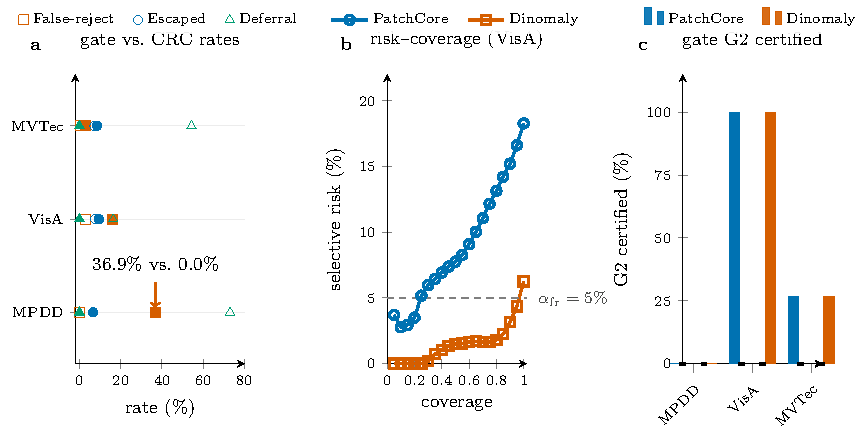
\includegraphics[width=0.62\linewidth]{../figures-src/fig-crcbaseline.pdf}
  \caption{Escaped-defect, false-reject, and deferral rates for our dual gate versus the
  single-threshold CRC baseline (Table~\ref{tab:crcbaseline}), pooled over both backbones and five
  seeds. CRC has no deferral mechanism, so every non-passed image becomes an auto-reject; on MPDD
  this drives its false-reject rate to $36.9\%$ against $0.0\%$ for our gate at the same
  escaped-defect rate.}
  \label{fig:crcbaseline}
\end{figure}
\FloatBarrier

As a second, non-conformal reference line we also compute the field-standard selective-prediction
risk-coverage curve~\citep{geifman2017selective} (per-category best-F1 threshold, margin-based
abstention) on the same score dumps. Its area-under-the-risk-coverage-curve (AURC, lower is
better) ranges from $0.0019$ (MVTec AD, Dinomaly) to $0.0849$ (VisA, PatchCore); at $\sim\!80\%$
coverage the realized risk is $0.0625$/$0.0154$ (MPDD, PatchCore/Dinomaly), $0.1315$/$0.0180$
(VisA, PatchCore/Dinomaly), and $0.0095$/$0.0026$ (MVTec AD, PatchCore/Dinomaly). This is a
fundamentally different guarantee --- a curve traced out by sweeping coverage post hoc, not a fixed
pre-specified certificate at a chosen risk level --- so we report it as context rather than a
like-for-like comparison to Table~\ref{tab:crcbaseline}.
% source: baseline_comparison_2026-07-15/results.json (selective_baseline, per-backbone aurc + risk_at_coverage[coverage=0.8])

\subsection{Latency and deployment cost}
\label{sec:latency}

The gate is a thin decision layer on top of whatever detector already produces the anomaly score,
so the only cost it adds is the conformal calibration (once, per calibration refresh) and the
per-image routing comparison. We measured both on this work's hardware, and we place them
alongside the backbone forward pass that dominates the end-to-end budget
(Table~\ref{tab:latency}). Routing an image is an $O(1)$ threshold comparison inside an
$O(\text{sort})$ calibration; the measured per-image routing cost is $2.8\,\mu$s on CPU ---
roughly four orders of magnitude below the backbone forward pass and under $0.02\%$ of Dinomaly's
per-image GPU inference. Calibrating the full three-way gate over one $861$-image calibration half
across all $15$ MVTec strata (the $\alpha_{\text{miss}}=0.10$, $\alpha_{\text{fr}}=0.05$ primary
configuration) takes $2.4$ ms end to end, and is amortized over an entire evaluation run rather
than paid per image. The practical conclusion for a manufacturing reader is that certification is
free relative to detection: a line already able to afford the detector can add the escaped-defect /
false-reject certificate at no measurable latency cost. The backbone rows are the honest budget the
gate sits on --- Dinomaly measured here on an RTX~5090 Laptop GPU, PatchCore's row taken from the
authors' reported figure (not measured here, and both hardware- and coreset-dependent). We flag the
substrate mix these numbers span, so no cross-row comparison is over-read: the gate rows are timed
on CPU over the MVTec calibration scores ($861$-image cal half, $15$ strata), the Dinomaly backbone
row on GPU over $250$ real VisA test images (the VisA branch-A seed-$0$ checkpoint), and the
PatchCore row is the authors' published $\sim$1\%-coreset figure whereas our scoring uses the
$10\%$-coreset configuration --- so the table brackets the order of magnitude of the
backbone budget the gate rides on, and it is the $\mu$s-scale CPU gate overhead, not any
CPU-vs-GPU or MVTec-vs-VisA backbone comparison, that the paper contributes.
% source: latency_2026-07-13/gate_latency.json (gate rows, measured CPU;
% Intel Core Ultra 9 275HX / 24 threads / 62 GB);
% latency_2026-07-13/dinomaly_latency.json (Dinomaly row, measured RTX 5090 Laptop GPU,
% torch 2.12.0+cu130, VisA branch-A seed-0 checkpoint, 250 real VisA test images);
% PatchCore row attributed to Roth et al. 2022 (published, not measured).
% KEEP (directive #2 remedy d): checked gate_latency.json/dinomaly_latency.json for
% per-category/per-seed rows to expand into -- none exist beyond these 2 single-point gate
% measurements (calibrate/route) and 2 backbone figures; this is the full granularity the
% frozen measurements support, so the 4-row table is load-bearing as-is (no merge partner
% exists either -- no other latency table in the paper).

\begin{table}[t]
  \centering
  \small
  \caption{Per-image latency and deployment cost. The two gate rows and the Dinomaly backbone row
  are \emph{measured on this work's hardware} (gate: Intel Core Ultra~9 275HX CPU, $24$ threads;
  Dinomaly: NVIDIA RTX~5090 Laptop GPU, torch~2.12.0, batch~$1$, median over $250$ real VisA test
  images, full forward\,$+$\,anomaly-map\,$+$\,image-score pass). The PatchCore backbone row is
  \emph{reported by the authors} (not measured here; \citealp{roth2022patchcore}, $\sim$1\%-coreset
  configuration on their hardware) and is included only to bracket the backbone budget --- backbone
  timing is hardware- and configuration-dependent, whereas the gate overhead below it is the
  measured constant this paper contributes. Sources: the frozen latency measurement dumps.}
  % source: latency_2026-07-13/{gate,dinomaly}_latency.json
  \label{tab:latency}
  \small
  \begin{tabular}{@{}>{\raggedright\arraybackslash}p{0.34\textwidth} l >{\raggedright\arraybackslash}p{0.34\textwidth}@{}}
    \toprule
    Component & Per-image cost & Notes \\
    \midrule
    \multicolumn{3}{@{}l}{\emph{Backbone forward pass (dominates the budget)}} \\
    \quad Dinomaly (DINOv2-b, $148$M) --- measured, GPU & $18.9$ ms (p95 $23.1$) & $53$ img/s at batch $1$; $17.0$ ms/img batched ($B{=}32$) \\
    \quad PatchCore (WRN50, coreset) --- \emph{authors' figure} & $\lesssim 200$ ms & \citet{roth2022patchcore}, their hardware; not measured here \\
    \midrule
    \multicolumn{3}{@{}l}{\emph{Gate overhead added on top (this paper) --- measured, CPU}} \\
    \quad Routing (per image) & $2.8\,\mu$s & $O(1)$ compare; $<0.02\%$ of the Dinomaly forward pass \\
    \quad Calibration (one-time) & $2.4$ ms (p95 $2.8$) & full $3$-way gate, $861$-img cal half, $15$ strata; per refresh \\
    \bottomrule
  \end{tabular}
\end{table}
\FloatBarrier

\section{Limitations and gated arms}
\label{sec:limitations}

The preregistration was frozen on 2026-07-11 (a sha256-pinned sign-off record over the
preregistration document and its A1--A3 amendments). One frozen arm
% freeze: SIGN-OFF-RECORD-2026-07-11.md pinned to PREREG-DRAFT-2026-07-10.md
has since been computed and is reported above (the G2 train-holdout promotion,
Section~\ref{sec:g2promo}). The VisA and MPDD benchmarks are both post-freeze additions ---
the frozen preregistration mentions neither --- run under the identical frozen protocol and
code path but reported as exploratory, never confirmatory, throughout
Section~\ref{sec:results}; MPDD's train-holdout rescue (Section~\ref{sec:mpddholdout}) is
additionally a flag-gated, prereg-neutral protocol variant. The following arms remain
\emph{unlocked but not yet computed}; each is
stated explicitly and is not reported as a result anywhere above.

\begin{itemize}
  \item \textbf{Confirmatory audit family (C2).} Now computed and reported
        (Section~\ref{sec:c2}, Table~\ref{tab:c2}): the four-member per-seed Holm family rejects the
        random-deferral null in all five seeds on MVTec AD --- a constructive verdict, every
        bootstrap CI excluding zero. The single cross-seed rollup was authored post-freeze as a
        one-shot reduction but is moot, the per-seed confirmatory verdict being unanimous across
        seed-min, seed-median, and seed-max.
  \item \textbf{B3 (train-good quantile) practice.} Now completed post-hoc for PatchCore
        (Section~\ref{sec:c2}): the confirmatory family treats B3's absence as the preregistered
        six-to-four degradation (PREREG~\S4), and, since a held-out train-good score pool exists for
        PatchCore, its B3 arm is reported post-hoc --- constructive in all five seeds, consistent
        with B1/B2. B3-Dinomaly remains impossible (no train-side score dump), so the full
        six-member family cannot be run; on VisA no train-good scores were dumped for either
        backbone, so B3 is unavailable there.
        % held-out train-good score dump exists for PatchCore (MVTec); none for Dinomaly or VisA
        % source: b3_patchcore_2026-07-13/
  \item \textbf{V1 tier-2 as a verdict.} Now graded (Section~\ref{sec:tier2verdict},
        Table~\ref{tab:tier2}):
        under amendments A1/A2/A3 the MVTec escaped axis fails in $115/130$
        powered cells --- the A2-expected estimator-variance behaviour, not a certificate failure,
        with tier-1 passing all $150$ cells --- and the false-reject axis is structurally ungraded
        ($0/150$; A1$+$A3). Its $+3$pp tolerance is near-unpassable for a correctly-calibrated gate
        by construction. VisA (exploratory) is partially gradeable on both axes.
  \item K6 (scoop re-scan). Now executed. The pre-submission citation re-scan for any prior
        certified three-way triage on MVTec AD or VisA was run fresh on 2026-07-13 and returned a
        clear verdict --- no scoop (Section~\ref{sec:related}), so the pre-decided pivot to the
        C2/C3-primary framing was not triggered. K6 is a \emph{novelty} gate, not a statistical one:
        it gates on no frozen result, so it is correctly run last, immediately before submission.
        The 2026-07-11 freeze therefore predates this execution by design; running K6 after the
        freeze is the intended sequencing, not an inconsistency.
        % source: analysis_2026-07-10/K6-RESCAN-2026-07-13.md
  \item K4 (audit headroom). K4 requires an oracle-headroom
        statistic the certification module does not yet implement.
        % K4 statistic to be added to certify.py
  \item \textbf{Remaining tables and figures.} The confirmatory audit table (Table~\ref{tab:c2}, now
        including the VisA post-freeze exploratory rows) and the tier-2 verdict table
        (Table~\ref{tab:tier2}, now a per-category breakdown) are now included. The defect-type
        Mondrian coverage-debt map (MVTec only; VisA has no defect-type axis) and the train-holdout
        G2 delta figure remain to be produced.
\end{itemize}

The latency and practicality figures an industrial-inspection reader will reasonably want are now
computed and reported in Section~\ref{sec:latency} (Table~\ref{tab:latency}): the gate adds a
measured $2.8\,\mu$s/image on CPU on top of the backbone forward pass, confirming the
$O(\text{sort})$ ``negligible'' claim with a real measurement rather than an argument.

Two non-gated caveats are also worth stating plainly.

\paragraph{Substrate maturity on MVTec AD, and what VisA settles.} Both reproduced backbones sit
near ceiling on MVTec AD (mean image-AUROC $0.982$ PatchCore, $0.996$ Dinomaly), and Dinomaly is
saturated enough per category that the exploratory excess-AURC audit has almost no headroom to
detect practice skill on it there --- its MVTec ``$0/30$ reject'' (with $14/30$ degenerate cells)
is uninformative about practice quality rather than evidence against it. The pre-freeze
skeleton's designed answer was a lower-ceiling second benchmark (stated there as a plan; VisA is
not part of the frozen preregistration), and it behaved as designed: on VisA
(Section~\ref{sec:auditres}) the same audit has zero degenerate cells and rejects the
random-deferral null in $14/24$ (PatchCore) and $16/24$ (Dinomaly) seed-$0$ practice-cells. The
confirmatory pooled audit (Section~\ref{sec:c2}) settles the deferral-skill question on MVTec AD
in the constructive direction, and the post-hoc binding demonstration (Section~\ref{sec:binding})
exhibits the still-sharper event directly: (backbone, category) cells where a naive fixed
threshold's realized escaped-defect or false-reject rate violates $\alpha_{\text{miss}}$ or
$\alpha_{\text{fr}}$ while the certified gate holds within target on the same data --- the event the
excess-AURC audit does not itself test. We
also state plainly that all three benchmarks are academic: no production-line, temporal-drift, or
real-factory data backs the industrial framing here (threshold-transfer across production
periods is future work), so the paper's claims are about certified triage on the standard
inspection benchmarks, not about a deployed line.

\paragraph{Small good-calibration pools are intended behavior, not a shortfall.} Under the primary
protocol, G2's $4/15$ certifiable count is a property of MVTec AD's test-good counts; honestly
reporting it (Table~\ref{tab:floors}) is the designed behavior, not a defect to be engineered
away outside the frozen calibration-efficiency remedy (Section~\ref{sec:g2promo}), and VisA's
$12/12$ under the identical arithmetic (with the identical code path) shows the refusals track
the data, not a conservatism baked into the gate. MPDD makes the same point at the opposite
extreme: its $0/6$ primary-protocol G2 count is the honest, data-limited behaviour of uniformly
small test-good pools, and the flag-gated train-holdout arm rescues it to $4/6$ (one category
KS-audited out; Section~\ref{sec:mpddholdout}), so the three benchmarks together give three points
consistent with pool-size-driven refusal ($0/6 \to 4/15 \to 12/12$). MPDD is
post-freeze exploratory and its train-holdout rescue is PatchCore-only (Dinomaly dumps no
train-side scores), disclosed as such and never entering the confirmatory family.

\section{Conclusion}
\label{sec:conclusion}

We described a certified three-way triage gate that turns any anomaly detector's scores into an
auditable inspection decision with finite-sample escaped-defect and false-reject guarantees, and a
refusal mechanism that makes ``not enough data to certify'' a visible outcome. On MVTec AD,
VisA, and MPDD, across two backbones and five seeds each, the calibration machinery matches its
preregistered arithmetic exactly, with no kill-gate tripped in any of the $30$ (backbone, seed)
aggregates. The three benchmarks exercise complementary failure modes and together give three
points consistent with pool-size-driven refusal ($0/6 \to 4/15 \to 12/12$): MVTec AD
stresses the refusal side (G2 certifiable in only $4/15$ categories under the primary protocol,
lifted to $12$--$13/15$ by the frozen train-holdout remedy --- PatchCore-only by data availability
--- with KS-failing categories honestly refused);
VisA --- lower-ceiling, larger good pools --- certifies both axes in all $12$ categories,
cuts median deferral to $4$--$19\%$, and gives the excess-AURC audit the headroom MVTec's
saturated backbones deny it; and MPDD (real painted-metal parts, post-freeze exploratory) is the
stingy extreme, refusing G2 in all $6$ categories under the primary protocol and rescued to $4/6$
by the flag-gated train-holdout arm (one category KS-audited out). The confirmatory pooled audit
(C2) returns a constructive verdict on
MVTec AD --- field-standard threshold practice earns real deferral skill over honest random deferral
in all five backbone seeds (Section~\ref{sec:c2}).

% =====================================================================
% Springer/JIM DECLARATIONS. Required by the journal; several fields are
% author-completed at submission (marked TODO-USER). At the sn-jnl drop-in these
% move under the template's declarations convention (\bmhead{Declarations}).
% The Data/Code availability text below is ported byte-faithfully from the
% "Data and code availability" section of ../paper.tex.
% =====================================================================
\section*{Declarations}

\paragraph{Funding.} \userfill{funding sources for this work, or the standard
statement ``The authors declare that no funds, grants, or other support were received during the
preparation of this manuscript.''}

\paragraph{Competing interests.} \userfill{declare any competing financial or
non-financial interests, or the standard statement ``The authors have no relevant financial or
non-financial interests to disclose.''}

\paragraph{Ethics approval.} Not applicable. This study uses only public benchmark datasets
(MVTec AD, VisA, and MPDD) and involves no human participants, animal subjects, or personally
identifiable data.

\paragraph{Data availability.} All three benchmarks are public: MVTec AD~\citep{bergmann2019mvtec},
VisA~\citep{zou2022spot}, and MPDD~\citep{jezek2021mpdd} (staged from the credential-free
HuggingFace mirror \texttt{meksamiao/mpdd}, archive sha256 \texttt{69f8da73\ldots ddd6} recorded in
the frozen split manifest). The frozen analyses that produced every reported number read only local
score dumps and are archived together with those dumps, the frozen preregistration, and its
sha256-pinned sign-off record. \userfill{a Zenodo DOI for the frozen score dumps and
analysis archive will be minted at submission under the author's deposit credentials.}
% archived score dumps: fullscore_results_2026-07-10/, dinomaly_brancha_2026-07-10/canonical/,
%   holdout_results_2026-07-10/, and the 2026-07-12 VisA pull
% analysis stages: analysis_2026-07-10/ -> SUMMARY.json (+ANALYSIS-MEMO.md; MVTec AD),
%   g2_promotion_2026-07-12/ -> G2-PROMOTION-RESULT.json,
%   visa_results_2026-07-12/ -> SUMMARY.json (+MVTEC-VS-VISA.md)
% preregistration PREREG-DRAFT-2026-07-10.md frozen 2026-07-11 (SIGN-OFF-RECORD-2026-07-11.md)

\paragraph{Code availability.} The gate is implemented in \emph{inspect-gate}, a thin wrapper
over the project's reliability metrics library; the frozen MVTec AD, G2-promotion, and VisA
analysis scripts that regenerate every reported summary are archived with the code. Per Springer
Nature's code-sharing policy, a bare repository link does not by itself carry a permanent
identifier, so the source will be maintained on GitHub as the development mirror and archived on
Zenodo under a persistent DOI. \userfill{GitHub repository URL, Zenodo DOI, and open-source
license to be provided at submission.}
% analysis scripts: analysis_2026-07-10/scripts/run_analysis.py -> SUMMARY.json;
%   g2_promotion_2026-07-12/run_g2_promotion.py -> G2-PROMOTION-RESULT.json;
%   visa_results_2026-07-12/scripts/visa_adapter.py + run_visa_analysis.py -> SUMMARY.json, MVTEC-VS-VISA.md
% code-archive policy: docs/records/CODE-ARCHIVE-POLICY-2026-07-16.md (JIM row: GitHub alone
% insufficient per Springer Nature's live code policy; pair with Zenodo/Code Ocean DOI)

\paragraph{Author contributions.} \userfill{e.g., ``Z.F. conceived the method, implemented the
gate and analysis, and wrote the manuscript.'' Adjust to the final author list.}

% Author-year reference style (plainnat, natbib round option) for the article-class
% port, matching JIM's live house style (verified 2026-07-16; see the natbib
% \usepackage comment above). At the sn-jnl drop-in, switch to
% \bibliographystyle{sn-basic} in its default author-year mode -- NOT its numbered
% variant.
\bibliographystyle{plainnat}
\bibliography{refs}

\end{document}
